\index{numerical stability}
\chapter{Numerical Stability in Deep Learning}
\printchapterversion{7_numerical_stability}
\newthought{Preventing NaN, Inf, and Mysterious Training Failures}


% ==============================================================================================
% INTRODUCTION BLOCK

\section{The Why}
\index{training failures}

\newthought{In the previous chapter,} we learned how to find global optima in complex loss landscapes.
The theory is elegant: search the space, find good minima, optimize.
But there is a gap between theory and practice: training can fail in mysterious ways.

\newthought{Common failure modes:}
\begin{itemize}
    \item Loss suddenly becomes NaN or Inf after training seemed fine for hours
    \item Gradients explode to $10^{30}$ or vanish to $10^{-30}$
    \item Training stalls with no progress despite non-zero gradients
    \item Outputs become degenerate: all zeros, all ones, or identical for every input
    \item Model predictions suddenly become random after many epochs
\end{itemize}

\marginnote{\newthought{Every deep learning framework} has stability tricks built in. When you use \texttt{torch.nn.functional.log\_softmax}, you are using the log-sum-exp trick. When you use \texttt{torch.nn.init.kaiming\_normal\_}, you are using He initialization. Understanding why these matter helps you debug when things go wrong.}

\newthought{The root cause:} Floating-point arithmetic has finite precision (Chapter 2). Operations that are mathematically equivalent can have vastly different numerical behavior. $\log(\exp(x)/\sum\exp(x_j))$ equals $x - \log\sum\exp(x_j)$, but the first overflows while the second doesn't.

\newthought{In machine learning and artificial intelligence,} numerical stability appears at every turn:
\begin{itemize}
    \item log\_softmax vs log(softmax): one works, one overflows for large logits
    \item Gradient clipping prevents exploding gradients in RNNs and transformers
    \item Weight initialization keeps activations in a reasonable range through many layers
    \item Mixed precision training gives 2$\times$ memory savings and speedup, but needs careful handling
    \item BatchNorm/LayerNorm normalizes activations to prevent drift
\end{itemize}

\newthought{The payoff:} Understanding numerical stability = debugging 90\% of ``training doesn't converge'' issues.



\newpage
\subsection{Hands On Experience}
\index{hands-on} \index{overflow}

\newthought{Consider computing} $\log\left(\sum_{i=1}^{n} e^{x_i}\right)$ with $x = [1000, 1001, 1002]$.

This expression appears everywhere: cross-entropy loss, softmax, attention scores.

\begin{marginfigure}
    \centering
    \begin{tikzpicture}
        \begin{axis}[
            width=5cm,
            height=5cm,
            axis lines=left,
            xlabel={$x$},
            ylabel={$e^x$},
            xmin=0, xmax=750,
            ymin=0, ymax=1.8e308,
            tick style={gray},
            label style={gray},
            axis line style={gray},
            ytick={0, 1e308},
            yticklabels={$0$, $10^{308}$},
            xtick={0, 350, 709},
            xticklabels={$0$, $350$, $709$},
        ]
        % Exponential curve
        \addplot[black, thick, smooth, domain=0:709, samples=80] {exp(x)};
        % FP64 max line
        \draw[gray, dashed] (axis cs:0, 1.7977e308) -- (axis cs:750, 1.7977e308);
        \node[gray, anchor=south west, font=\scriptsize] at (axis cs:10, 1.7977e308) {FP64 max};
        % Overflow marker
        \draw[gray, dotted] (axis cs:709, 0) -- (axis cs:709, 1.7977e308);
        \end{axis}
    \end{tikzpicture}
    \caption{The exponential function reaches the FP64 limit ($\approx 1.8 \times 10^{308}$) at $x \approx 709$. Beyond this, $e^x$ returns Inf.}
    \label{fig:exp_overflow}
\end{marginfigure}

\vspace{1em}
\newthought{Naive approach:}
\begin{align*}
    e^{1000} &\approx 10^{434} \quad \text{(overflow! FP64 max $\approx 10^{308}$, returns Inf)} \\
    e^{1001} &= \text{Inf} \\
    e^{1002} &= \text{Inf} \\
    \sum e^{x_i} &= \text{Inf} + \text{Inf} + \text{Inf} = \text{Inf} \\
    \log(\text{Inf}) &= \text{Inf}
\end{align*}

But wait---the true answer is $\log(e^{1000} + e^{1001} + e^{1002}) \approx 1002.4$, which is perfectly representable in floating point!

\marginnote{\newthought{The insight:} The problem is not the final answer---it is the intermediate computation. By reformulating, we avoid ever computing the huge intermediate values.}

\vspace{1em}
\newthought{Stable approach} (log-sum-exp trick):
\begin{align*}
    m &= \max(x) = 1002 \\
    x - m &= [1000-1002, 1001-1002, 1002-1002] = [-2, -1, 0] \\
    e^{-2} + e^{-1} + e^{0} &= 0.135 + 0.368 + 1.000 = 1.503 \\
    \log(1.503) &= 0.407 \\
    \text{Result:} \quad m + 0.407 &= 1002.407 \quad \checkmark
\end{align*}

Same mathematical result, no overflow! By shifting all values by the maximum, the largest exponent becomes 0, and all others are negative (hence safe).

\marginnote{\newthought{Compare with Chapter~2:} We saw that floating-point numbers have finite range. The same limitation that causes $10^{400}$ to overflow now causes $e^{1000}$ to overflow. The log-sum-exp trick is a direct response to the finite exponent range of IEEE 754.}

\vspace{1em}
\newthought{Why $\max(x)$?} Using the maximum ensures:
\begin{itemize}
    \item At least one term $e^{x_i - m} = e^0 = 1$ (no underflow to zero)
    \item All other terms $e^{x_i - m} \leq 1$ (no overflow)
\end{itemize}


\vspace{2.5em}
\newthought{The Learning Objectives} of this chapter aim at providing you with the abilities to:
\begin{itemize}
    \item Apply the log-sum-exp trick to prevent overflow in cross-entropy and attention
    \item Implement numerically stable softmax and understand why frameworks do it automatically
    \item Use gradient clipping to prevent exploding gradients in deep/recurrent networks
    \item Choose appropriate weight initialization (Xavier, He) based on activation function
    \item Understand mixed precision training (FP16, BF16) and when to use it
    \item Recognize and diagnose numerical stability issues in training
\end{itemize}




% ==============================================================================================
% MAIN THEORY BLOCK

\newpage
\section{Stable Computations}
\index{log-sum-exp}

\subsection{The Log-Sum-Exp Trick}

\newthought{The problem:} Computing $\log\sum_i e^{x_i}$ naively causes overflow when any $x_i$ is large (say, $> 700$ for FP64).

\newthought{The identity:} For any constant $c$:
\begin{equation}
    \log\sum_{i=1}^{n} e^{x_i} = c + \log\sum_{i=1}^{n} e^{x_i - c}
\end{equation}

\newthought{Proof:}
\begin{align}
    \log\sum_i e^{x_i} &= \log\left(e^c \cdot \sum_i e^{x_i - c}\right) \\
    &= \log(e^c) + \log\sum_i e^{x_i - c} \\
    &= c + \log\sum_i e^{x_i - c}
\end{align}

\newthought{The solution:} Choose $c = m = \max_i x_i$:
\begin{equation}
    \log\sum_{i=1}^{n} e^{x_i} = m + \log\sum_{i=1}^{n} e^{x_i - m}
\end{equation}

\marginnote{\newthought{Why $\max$?} With $c = \max(x)$:
\begin{itemize}
    \item Largest exponent becomes $e^0 = 1$ (no overflow)
    \item All exponents are $\leq 0$ (bounded by 1)
    \item Sum is $\geq 1$ (no underflow to 0)
\end{itemize}}

\begin{algorithm}[H]
\caption{Numerically Stable Log-Sum-Exp}
\begin{algorithmic}[1]
    \Require Input vector $x = [x_1, x_2, \ldots, x_n]$
    \State Find maximum: $m \gets \max_i x_i$
    \State Shift values: $x' \gets x - m$
    \State Compute safe sum: $S \gets \sum_{i=1}^{n} e^{x'_i}$
    \State Add back maximum: result $\gets m + \log(S)$
    \Return result
\end{algorithmic}
\end{algorithm}

\newthought{This is used in} cross-entropy loss, attention, and beyond:
\begin{itemize}
    \item Cross-entropy loss: $-\log p_y = -\log\text{softmax}(x)_y = -x_y + \log\sum_j e^{x_j}$
    \item Attention scores: $\text{softmax}(QK^T / \sqrt{d})$ with large $QK^T$ values
    \item Energy-based models: partition functions $Z = \sum_x e^{-E(x)}$
    \item Probabilistic models: log-likelihoods, marginal probabilities
\end{itemize}


\newthought{Numerical comparison:}

\vspace{2em}
\begin{table*}[ht]
\centering
\begin{tabular*}{\textwidth}{@{\extracolsep{\fill}}p{0.22\textwidth}p{0.28\textwidth}p{0.25\textwidth}p{0.25\textwidth}}
\toprule
\textbf{Input} & \textbf{True Value} & \textbf{Naive} & \textbf{Log-sum-exp} \\
\midrule
$[1, 2, 3]$ & 3.41 & 3.41 & 3.41 \\
$[100, 101, 102]$ & 102.41 & 102.41 & 102.41 \\
$[1000, 1001, 1002]$ & 1002.41 & Inf & 1002.41 \\
$[-1000, -999, -998]$ & $-997.59$ & $-\infty$ & $-997.59$ \\
$[0, 0, 0]$ & 1.10 & 1.10 & 1.10 \\
\bottomrule
\end{tabular}
\vspace{2em}
\caption{Numerical comparison of naive vs.\ log-sum-exp computation for various inputs.}
\label{tab:logsumexp_comparison}
\end{table*}

The stable version handles extreme values that would destroy the naive computation.




\subsection{Stable Softmax and Log-Softmax}
\index{softmax!stable}

\newthought{The softmax function} converts arbitrary real numbers (logits) to probabilities:
\begin{equation}
    \text{softmax}(x)_i = \frac{e^{x_i}}{\sum_j e^{x_j}}
\end{equation}

Properties: All outputs in $(0, 1)$, sum to 1, preserves ordering.

\marginnote{\newthought{Softmax is the continuous analogue} of argmax. As a ``temperature'' parameter $\tau \to 0$, $\text{softmax}(x/\tau)$ approaches a one-hot vector---but the intermediate values grow as $1/\tau$, making stability critical.}

\subsection{The Overflow Problem}
\index{overflow}

\newthought{Naive implementation:}
\begin{align*}
    x &= [1000, 1001, 1002] \\
    e^{x} &= [\text{Inf}, \text{Inf}, \text{Inf}] \\
    \text{sum} &= \text{Inf} \\
    \text{softmax}(x) &= [\text{Inf}/\text{Inf}, \text{Inf}/\text{Inf}, \text{Inf}/\text{Inf}] = [\text{NaN}, \text{NaN}, \text{NaN}]
\end{align*}

The computation fails even though the true answer is $[0.09, 0.24, 0.67]$---perfectly normal probabilities!


\subsection{The Stable Solution}
\index{numerical stability}

\newthought{Key observation:} Softmax is shift-invariant:
\begin{equation}
    \text{softmax}(x)_i = \text{softmax}(x - c)_i \quad \text{for any constant } c
\end{equation}

\newthought{Proof:}
\begin{equation}
    \frac{e^{x_i - c}}{\sum_j e^{x_j - c}} = \frac{e^{x_i} / e^c}{\sum_j e^{x_j} / e^c} = \frac{e^{x_i}}{\sum_j e^{x_j}}
\end{equation}

\newthought{Stable softmax:}
\begin{equation}
    \text{softmax}(x)_i = \frac{e^{x_i - m}}{\sum_j e^{x_j - m}}, \quad m = \max_j x_j
\end{equation}

\marginnote{\newthought{In code:}
\begin{verbatim}
# Unstable (don't use!)
p = np.exp(x) / np.sum(np.exp(x))

# Stable
m = np.max(x)
p = np.exp(x - m) / np.sum(np.exp(x - m))

# Or just use the built-in
p = torch.softmax(x, dim=-1)
\end{verbatim}}


\subsection{Log-Softmax: Combining Stability}
\index{log-softmax}

\newthought{Cross-entropy loss} requires $\log(\text{softmax}(x))$. Computing softmax then log loses precision:

\begin{equation}
    \text{softmax}(x)_i = 0.0000001 \quad \Rightarrow \quad \log(0.0000001) = -16.1
\end{equation}

For very confident predictions, softmax gives numbers very close to 0 or 1, which lose precision before the log.

\newthought{Direct log-softmax:}
\begin{align}
    \log\text{softmax}(x)_i &= \log\frac{e^{x_i}}{\sum_j e^{x_j}} \\
    &= x_i - \log\sum_j e^{x_j} \\
    &= x_i - m - \log\sum_j e^{x_j - m}
\end{align}

This is what \texttt{torch.nn.functional.log\_softmax} computes---numerically stable and more accurate than \texttt{log(softmax(x))}.




\subsection{Gradient Clipping}
\index{gradient clipping}

\newthought{The problem:} During training, gradients can become extremely large, causing:
\begin{itemize}
    \item Enormous parameter updates that overshoot any reasonable minimum
    \item Numerical overflow (Inf values) in parameters or activations
    \item Training instability: loss jumps around wildly or goes to NaN
\end{itemize}

\marginnote{\newthought{Exploding gradients} are especially common in:
\begin{itemize}
    \item RNNs (gradients multiply through time)
    \item Very deep networks
    \item Transformers (large attention scores)
    \item Reinforcement learning
\end{itemize}}

\newthought{Root cause in RNNs:} Gradients flow through $T$ time steps via:
\begin{equation}
    \frac{\partial L}{\partial h_0} = \frac{\partial L}{\partial h_T} \cdot \prod_{t=1}^{T} W^T
\end{equation}

If the spectral norm $\|W\| > 1$, gradients grow as $\|W\|^T$---exponentially!


\subsection{Clip by Value}
\index{clip by value}

The simplest approach: clamp each gradient component independently.
\begin{equation}
    g'_i = \text{clip}(g_i, -\tau, \tau) = \max(-\tau, \min(\tau, g_i))
\end{equation}

\newthought{The drawback} is that this can drastically change gradient direction. If $g = [1000, 1]$ and $\tau = 1$, then $g' = [1, 1]$---the direction completely changed.


\subsection{Clip by Norm (Preferred)}
\index{clip by norm}

Scale the entire gradient vector if its norm exceeds a threshold:
\begin{equation}
    g' = g \cdot \min\left(1, \frac{\tau}{\|g\|}\right) = \begin{cases} g & \text{if } \|g\| \leq \tau \\ \tau \cdot \frac{g}{\|g\|} & \text{if } \|g\| > \tau \end{cases}
\end{equation}

\newthought{The key properties} of clipping by norm are:
\begin{itemize}
    \item Direction is preserved: $g'$ points the same way as $g$
    \item The norm is bounded: $\|g'\| \leq \tau$ always
    \item Small gradients are unchanged: if $\|g\| \leq \tau$, no modification occurs
\end{itemize}

\begin{algorithm}[H]
\caption{Gradient Clipping by Norm}
\begin{algorithmic}[1]
    \Require Gradient vector $g$, threshold $\tau$
    \State Compute norm: $\text{norm} \gets \|g\|_2$
    \If{$\text{norm} > \tau$}
        \State Scale gradient: $g \gets g \cdot \tau / \text{norm}$
    \EndIf
    \Return $g$
\end{algorithmic}
\end{algorithm}

\begin{figure}[h]
    \centering
    \begin{tikzpicture}[scale=1.2]
        % Axes
        \draw[gray, ->] (-0.5, 0) -- (3.5, 0);
        \draw[gray, ->] (0, -0.5) -- (0, 2.5);
        % Threshold circle
        \draw[dashed, gray] (0, 0) circle (1.5);
        \node[gray, below right] at (1.5, 0) {$\tau$};
        % Original gradient
        \draw[->, thick, black] (0, 0) -- (3, 2);
        \node[right] at (3, 2) {$g$ (original)};
        % Clipped gradient
        \draw[->, thick, gray] (0, 0) -- (1.25, 0.833);
        \node[above left, gray] at (1.1, 0.9) {$g'$ (clipped)};
    \end{tikzpicture}
    \caption{Gradient clipping by norm: $g'$ has the same direction as $g$ but magnitude at most $\tau$.}
    \label{fig:gradient_clipping}
\end{figure}

\marginnote{\newthought{Typical values:} $\tau \in [0.5, 5]$. Start with $\tau = 1$ and adjust based on training behavior.
\begin{itemize}
    \item Too small: slow training
    \item Too large: no effect on explosions
\end{itemize}}

\newthought{When to use:} Apply gradient clipping if:
\begin{itemize}
    \item Training loss occasionally spikes dramatically
    \item You're training RNNs or very deep networks
    \item Training terminates with NaN after running fine for a while
\end{itemize}




\newpage
\section{Weight Initialization and Normalization}
\index{weight initialization}
\index{Xavier initialization}
\index{He initialization}

\newthought{The problem:} With bad initialization, activations can explode or vanish as they pass through layers. This makes early training unstable or impossible.


\subsection{Variance Propagation Analysis}
\index{variance propagation}

Consider a single layer $y = Wx$ where $W \in \mathbb{R}^{n_{\text{out}} \times n_{\text{in}}}$, with independent entries.

\begin{align}
    y_j &= \sum_{i=1}^{n_{\text{in}}} W_{ji} x_i \\
    \text{Var}(y_j) &= \sum_{i=1}^{n_{\text{in}}} \text{Var}(W_{ji} x_i) \\
    &= n_{\text{in}} \cdot \text{Var}(W) \cdot \text{Var}(x) \quad \text{(assuming zero mean, independence)}
\end{align}

\marginnote{\newthought{The goal:} Keep $\text{Var}(y) \approx \text{Var}(x)$ through all layers, so activations neither explode ($\to \infty$) nor vanish ($\to 0$).}

\newthought{To maintain variance:} We need $n_{\text{in}} \cdot \text{Var}(W) = 1$, so:
\begin{equation}
    \text{Var}(W) = \frac{1}{n_{\text{in}}}
\end{equation}


\subsection{Xavier/Glorot Initialization}
\index{Glorot initialization}

\newthought{For symmetric activations} (tanh, sigmoid near zero):

Glorot \& Bengio (2010) suggested balancing both forward and backward passes:
\begin{equation}
    W \sim \mathcal{N}\left(0, \frac{2}{n_{\text{in}} + n_{\text{out}}}\right)
\end{equation}

or equivalently, uniform on $\left[-\sqrt{\frac{6}{n_{\text{in}}+n_{\text{out}}}}, \sqrt{\frac{6}{n_{\text{in}}+n_{\text{out}}}}\right]$.

The average of $n_{\text{in}}$ and $n_{\text{out}}$ balances forward activation variance and backward gradient variance.


\subsection{He/Kaiming Initialization}
\index{Kaiming initialization}

\newthought{For ReLU activations,} which zero out half the inputs:

He et al. (2015) showed that ReLU reduces variance by half (since half the values become 0). To compensate:
\begin{equation}
    W \sim \mathcal{N}\left(0, \frac{2}{n_{\text{in}}}\right)
\end{equation}

The factor of 2 compensates for ReLU killing negative values.

\vspace{2em}
\begin{table*}[ht]
\centering
\begin{tabular}{p{0.26\textwidth}p{0.32\textwidth}p{0.20\textwidth}}
\toprule
\textbf{Activation} & \textbf{Variance} & \textbf{Name} \\
\midrule
Linear, tanh, sigmoid & $1/n_{\text{in}}$ or $2/(n_{\text{in}} + n_{\text{out}})$ & Xavier/Glorot \\
ReLU, Leaky ReLU & $2/n_{\text{in}}$ & He/Kaiming \\
SELU & Specific to activation & LeCun \\
\bottomrule
\end{tabular}
\vspace{2em}
\caption{Weight initialization strategies for different activation functions.}
\label{tab:weight_init}
\end{table*}

\marginnote{\newthought{In PyTorch:}
\begin{verbatim}
# Xavier
nn.init.xavier_normal_(w)
nn.init.xavier_uniform_(w)

# He/Kaiming
nn.init.kaiming_normal_(w)
nn.init.kaiming_uniform_(w)
\end{verbatim}}

\begin{figure}[h]
    \centering
    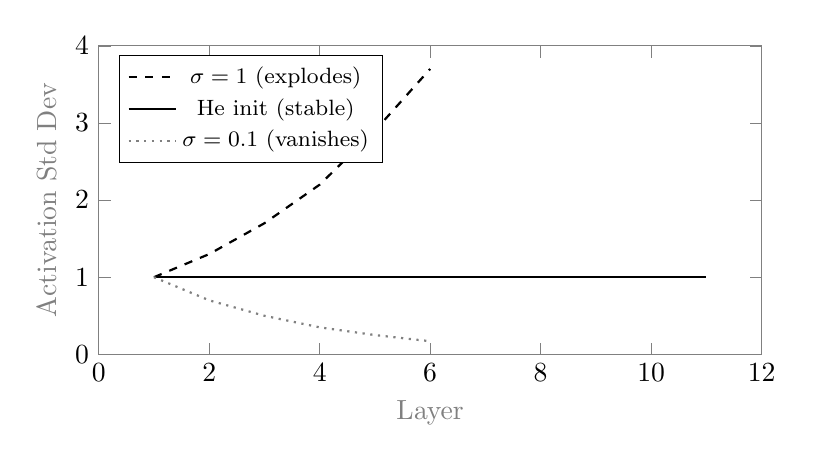
\begin{tikzpicture}
        \begin{axis}[
            width=10cm,
            height=5.5cm,
            xlabel={Layer},
            ylabel={Activation Std Dev},
            xmin=0, xmax=12,
            ymin=0, ymax=4,
            tick style={gray},
            label style={gray},
            axis line style={gray},
            legend pos=north west,
            legend style={font=\footnotesize},
        ]
        % Bad init (explodes)
        \addplot[black, thick, dashed] coordinates {(1, 1) (2, 1.3) (3, 1.7) (4, 2.2) (5, 2.9) (6, 3.7)};
        \addlegendentry{$\sigma = 1$ (explodes)}
        % Good init (stable)
        \addplot[black, thick] coordinates {(1, 1) (2, 1) (3, 1) (4, 1) (5, 1) (6, 1) (7, 1) (8, 1) (9, 1) (10, 1) (11, 1)};
        \addlegendentry{He init (stable)}
        % Bad init (vanishes)
        \addplot[gray, thick, dotted] coordinates {(1, 1) (2, 0.7) (3, 0.5) (4, 0.35) (5, 0.25) (6, 0.17)};
        \addlegendentry{$\sigma = 0.1$ (vanishes)}
        \end{axis}
    \end{tikzpicture}
    \caption{Activation standard deviation vs.\ layer depth for different initializations. Only properly scaled initialization keeps activations stable.}
    \label{fig:init_comparison}
\end{figure}




\subsection{Batch Normalization Numerics}
\index{batch normalization}

\newthought{Batch normalization} normalizes activations within a mini-batch to have zero mean and unit variance:
\begin{equation}
    \hat{x}_i = \frac{x_i - \mu_B}{\sqrt{\sigma_B^2 + \varepsilon}}
\end{equation}

where $\mu_B = \frac{1}{m}\sum_{i=1}^m x_i$ and $\sigma_B^2 = \frac{1}{m}\sum_{i=1}^m (x_i - \mu_B)^2$ are computed over the mini-batch.


\subsection{The Role of $\varepsilon$}
\index{epsilon}

\newthought{The $\varepsilon$ parameter} prevents division by zero:
\begin{itemize}
    \item A typical value is $\varepsilon = 10^{-5}$
    \item Without $\varepsilon$, if all inputs are identical, $\sigma_B^2 = 0$ and we divide by zero $\Rightarrow$ NaN
    \item Too large an $\varepsilon$ effectively removes the normalization effect
\end{itemize}

\marginnote{\newthought{When $\sigma_B^2 \approx 0$:} All inputs are nearly identical. This can happen:
\begin{itemize}
    \item Early in training with bad init
    \item In dying ReLU situations
    \item With very small batches
\end{itemize}}


\subsection{LayerNorm vs BatchNorm}
\index{layer normalization}

\newthought{LayerNorm} normalizes across features instead of across the batch:
\begin{equation}
    \hat{x}_i = \frac{x_i - \mu_L}{\sqrt{\sigma_L^2 + \varepsilon}}
\end{equation}

where statistics are computed over the feature dimension.

\vspace{2em}
\begin{table*}[ht]
\centering
\begin{tabular}{p{0.26\textwidth}p{0.26\textwidth}p{0.26\textwidth}}
\toprule
\textbf{Aspect} & \textbf{BatchNorm} & \textbf{LayerNorm} \\
\midrule
Normalize over & Batch dimension & Feature dimension \\
Used in & CNNs & Transformers, RNNs \\
Batch size dependency & Yes (needs $\geq$ 16-32) & No \\
Running statistics & Yes (for inference) & No \\
\bottomrule
\end{tabular}
\vspace{2em}
\caption{Comparison of BatchNorm and LayerNorm normalization approaches.}
\label{tab:batchnorm_layernorm}
\end{table*}




\newpage
\section{Mixed Precision Training}
\index{mixed precision}
\index{FP16}
\index{BF16}

\newthought{The idea:} Use lower precision (FP16 or BF16) for most operations, FP32 for critical parts. This exploits the fact that neural networks are remarkably tolerant of reduced precision.


\subsection{Benefits of Mixed Precision}
\index{mixed precision!benefits}

\newthought{The benefits} are substantial:
\begin{itemize}
    \item Memory: 2$\times$ reduction (16 bits vs 32 bits per number)
    \item Speed: 2-8$\times$ speedup on modern GPUs (tensor cores optimized for FP16)
    \item Scale: train larger models that would not fit in memory otherwise
\end{itemize}


\subsection{The Challenges}
\index{mixed precision!challenges}

\newthought{FP16 has limited range:} $\sim 6 \times 10^{-5}$ to $\sim 65504$.

\vspace{2em}
\begin{table*}[ht]
\centering
\begin{tabular*}{\textwidth}{@{\extracolsep{\fill}}p{0.25\textwidth}p{0.25\textwidth}p{0.25\textwidth}p{0.25\textwidth}}
\toprule
\textbf{Format} & \textbf{Exponent} & \textbf{Mantissa} & \textbf{Max Value} \\
\midrule
FP32 & 8 bits & 23 bits & $3.4 \times 10^{38}$ \\
FP16 & 5 bits & 10 bits & $6.5 \times 10^{4}$ \\
BF16 & 8 bits & 7 bits & $3.4 \times 10^{38}$ \\
\bottomrule
\end{tabular}
\vspace{2em}
\caption{Comparison of floating-point formats used in mixed precision training.}
\label{tab:fp_formats}
\end{table*}

\marginnote{\newthought{Typical issues:}
\begin{itemize}
    \item Gradients $< 10^{-5}$ underflow to 0
    \item Loss values $> 65504$ overflow to Inf
    \item Running sums accumulate error
\end{itemize}}


\subsection{Loss Scaling}
\index{loss scaling}

\newthought{Problem:} Small gradients underflow to zero in FP16.

\newthought{Solution:} Scale loss before backward pass, unscale gradients after.
\begin{align}
    \tilde{L} &= S \cdot L \quad \text{(scaled loss, compute backward in FP16)} \\
    \tilde{g} &= \nabla \tilde{L} = S \cdot \nabla L \quad \text{(scaled gradient)} \\
    g &= \tilde{g} / S \quad \text{(unscale in FP32 before optimizer step)}
\end{align}

Typical scale: $S = 2^{16}$ to $2^{24}$, adjusted dynamically if overflow detected.


\subsection{BF16: The Modern Alternative}
\index{BF16}

\newthought{BF16 (Brain Float 16)} keeps FP32's exponent range but truncates the mantissa:

\begin{itemize}
    \item It has the same range as FP32, so no overflow/underflow issues arise
    \item Less precision: 7 mantissa bits vs 23 (FP32) or 10 (FP16)
    \item Often no loss scaling is needed, as the range handles typical gradient magnitudes
\end{itemize}

BF16 is increasingly the default for large language model training---simpler and robust.




% ==============================================================================================
% STUDENT ACTIVATION BLOCK

\newpage
\section{Examples \& Exercises}
\index{exercises}

\marginnote{\newthought{Code} can be found at \url{https://github.com/Quillstacks/lecturecode_numericalmethods.git}.}

\newthought{Log-sum-exp by hand.} Compute $\log(e^{-100} + e^{-99} + e^{-98})$ using the log-sum-exp trick.

\begin{align*}
    m &= \max(-100, -99, -98) = -98 \\
    x - m &= [-100-(-98), -99-(-98), -98-(-98)] = [-2, -1, 0] \\
    e^{-2} + e^{-1} + e^{0} &= 0.135 + 0.368 + 1.000 = 1.503 \\
    \log(1.503) &= 0.407 \\
    \text{Result:} \quad -98 + 0.407 &= -97.593
\end{align*}

\marginnote{\newthought{Naive computation:} $e^{-100} + e^{-99} + e^{-98} \approx 0 + 0 + 0 = 0$ (underflow!), giving $\log(0) = -\infty$.}


\vspace{2em}
\newthought{Softmax stability.} Compute softmax of $x = [1000, 1000, 1000]$ both ways.
First try the naive approach: What is $e^{1000}$? What is $e^{1000}/(\text{Inf}+\text{Inf}+\text{Inf})$?
Then compute the stable version: What is $x - m$? What is $e^0 / (e^0 + e^0 + e^0)$?
Finally, reason about what the true answer should be by symmetry.


\vspace{2em}
\newthought{He initialization by hand.} For a layer with $n_{\text{in}} = 784$ inputs and $n_{\text{out}} = 256$ outputs using ReLU,
calculate the variance for He initialization $\text{Var}(W)$ and the corresponding standard deviation $\sigma$.
Then reason about what would happen if you initialized with $\sigma = 1$ instead---how would variance change per layer?

\marginnote{\newthought{Think about} what happens after 10 layers with the wrong initialization. How does the variance compound?}


\vspace{2em}
\newthought{Gradient clipping by hand.} A gradient has components $g = [3, 4]$ with $\|g\| = 5$. Compute the clipped gradient for $\tau = 2$.

\begin{align*}
    \|g\| &= \sqrt{3^2 + 4^2} = 5 > \tau \\
    \text{scale} &= \min(1, 2/5) = 0.4 \\
    g' &= 0.4 \cdot [3, 4] = [1.2, 1.6] \\
    \|g'\| &= \sqrt{1.2^2 + 1.6^2} = 2 = \tau \quad \checkmark
\end{align*}


\vspace{2em}
\newthought{Diagnosing instability.} Your training shows: loss is 0.5 for 1000 steps, then suddenly jumps to NaN. What techniques would you apply? In what order?




\newpage
\section{Self-Reflection and Recap}
\index{recap}

\newthought{Self-Reflection} Questions to guide your understanding:
\begin{itemize}
    \item Why does the $\varepsilon$ in BatchNorm matter? What specific failure does it prevent?
    \item When should you use gradient clipping? What symptoms indicate you need it?
    \item Why is mixed precision training not ``cheating''---what mathematical properties are preserved?
    \item How does initialization variance affect the ability to train very deep networks?
    \item Why does \texttt{log\_softmax} exist as a separate function rather than composing \texttt{log} and \texttt{softmax}?
    \item Could gradient clipping ever hurt training? When might you not want it?
\end{itemize}


\newthought{Recap} of Key Concepts:
\begin{itemize}
    \item Mathematically equivalent formulas can have very different floating-point behavior. Always prefer the stable version.
    \item The log-sum-exp trick $\log\sum e^{x_i} = m + \log\sum e^{x_i - m}$ prevents overflow/underflow.
    \item Stable softmax subtracts the maximum before exponentiating. Use \texttt{log\_softmax} for cross-entropy.
    \item Gradient clipping $g' = g \cdot \min(1, \tau/\|g\|)$ bounds gradient norm while preserving direction.
    \item Weight initialization: Xavier for tanh/sigmoid, He ($\text{Var} = 2/n_{\text{in}}$) for ReLU.
    \item Mixed precision uses FP16/BF16 for speed and FP32 master weights for precision. Use loss scaling with FP16.
\end{itemize}


\marginnote[2em]{\newthought{Teaser.} We can now train stably. But training minimizes expected loss---which is an integral over the data distribution. How do we compute integrals numerically?}

\newthought{From optimization to integration.} We have covered how to make neural network training numerically robust: stable softmax, gradient clipping, proper initialization, mixed precision. These techniques are built into every modern framework.

But we have been computing $\frac{1}{n}\sum_{i=1}^n L(x_i)$ as if it were obviously the right thing to do. This batch average is actually an approximation to an integral: $\mathbb{E}_{x \sim p}[L(x)] = \int L(x) p(x) dx$. How good is this approximation? Can we do better? In the next chapter, we will study numerical integration---the foundation for understanding why batch averaging works and when it might fail.



%%%%%%%%%%%%%%%%%%%%%%%%%%%%%%%%%%%%%%%%%%%%%%%%%%%%%%%%%%%%%%%%%%%%%%%%%%%%%%
